\documentclass[aspectratio=169]{beamer}
\usepackage{amsmath}
\usepackage{graphicx}
\usepackage{eso-pic} % Required for adding an image background
\usepackage{mdframed}

\title{Radiation and Shielding}
\author{By Ian Wald}
\date{\today}

\begin{document}

\frame{\titlepage}

\begin{frame}
\vspace{0.5cm}
\frametitle{Introduction to Radiation}
Radiation is the emission of energy as electromagnetic waves or as moving subatomic particles. It can be classified into four major types:
\begin{itemize}
    \item Alpha particles
    \item Beta particles
    \item Neutrons
    \item Electromagnetic waves (gamma rays and X-rays)
\end{itemize}
These types of radiation vary in mass, energy, and their ability to penetrate materials.
\end{frame}

\begin{frame}
\frametitle{Alpha Particles}
\begin{itemize}
    \item Consist of two protons and two neutrons
    \item Heaviest type of radiation particle
    \item Emitted by radioactive materials like uranium and thorium
    \item Example: Radon gas in homes
\end{itemize}
\end{frame}

\begin{frame}
\frametitle{Beta Particles}
\begin{itemize}
    \item Electrons not attached to atoms
    \item Small mass and negative charge
    \item Emitted by materials like tritium and carbon-14
    \item Used in applications like carbon dating and medical imaging
\end{itemize}
\end{frame}

\begin{frame}
\frametitle{Neutrons}
\begin{itemize}
    \item Uncharged particles found in atomic nuclei
    \item Commonly released during nuclear fission
    \item Essential for sustaining nuclear reactions in reactors
\end{itemize}
\end{frame}

\begin{frame}
\frametitle{Electromagnetic Radiation}
\begin{itemize}
    \item Includes gamma rays and X-rays
    \item No mass or charge
    \item High energy, capable of deep penetration
    \item Widely used in medical treatments and imaging
\end{itemize}
\end{frame}

\begin{frame}
\frametitle{Effects of Shielding}
\begin{itemize}
    \item \textbf{Alpha particles:}
    \begin{itemize}
        \item Stopped by a sheet of paper or skin
        \item However dangerous if inhaled or ingested
    \end{itemize}
    \item \textbf{Beta particles:}
    \begin{itemize}
        \item Require small amounts of shielding (plastic and glass)
        \item Can penetrate skin but not deeply into tissues
    \end{itemize}
    \item \textbf{Gamma rays and X-rays:}
    \begin{itemize}
        \item Require dense materials like lead or concrete
        \item Can penetrate deep into tissues and organs
    \end{itemize}
    \item \textbf{Neutrons:}
    \begin{itemize}
        \item Best shielded by materials with light atoms (like water) yet difficult.
        \item Can penetrate deeply due to being uncharged particles; it does interact with electrons and can penetrate deep into materials. 
    \end{itemize}
\end{itemize}
\end{frame}

\begin{frame}
    \frametitle{A Visualized Representation}
    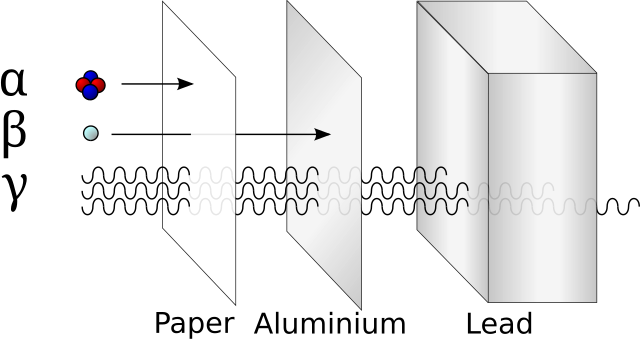
\includegraphics[width=1\textwidth]{images/Alfa_beta_gamma_radiation_penetration.svg.png}
\end{frame}

\begin{frame}
    \frametitle{Radiation Detectors}
    \begin{minipage}{0.32\textwidth}
        \centering
        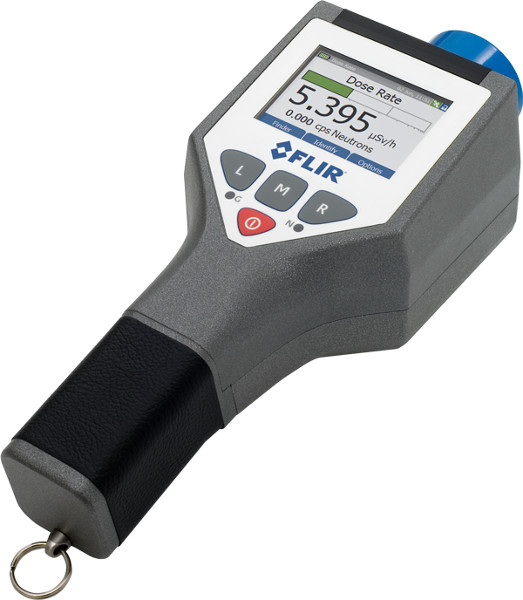
\includegraphics[width=\textwidth]{images/identifinder-r400.jpg}
    \end{minipage}
    \begin{minipage}{0.32\textwidth}
        \centering
        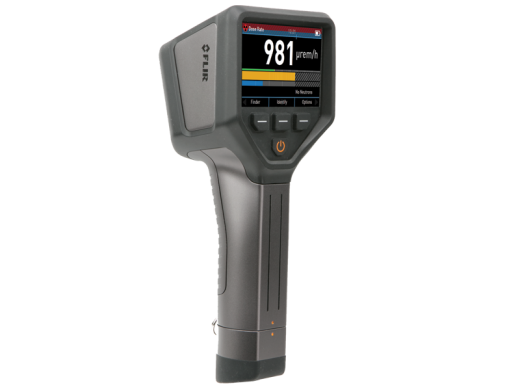
\includegraphics[width=\textwidth]{images/3ec8b23336eae1f156ba18f4e28166bd.1624378760.png}
    \end{minipage}
    \begin{minipage}{0.32\textwidth}
        \centering
        
\includegraphics[width=\textwidth]{images/trans-spec-n.png}
    \end{minipage}
\end{frame}

\begin{frame}
    \frametitle{Conclusion}
    \begin{itemize}
        \item Radiation comes in various forms with distinct properties and uses.
        \item Understanding the types and effects of radiation helps in safely harnessing its benefits while minimizing risks.
        \item Effective shielding is crucial in protecting against harmful radiation exposure.
    \end{itemize}
\end{frame}

\end{document}